\section{Introduction}

\subsection{Background and motivation}

A fault-tolerant quantum computer must protect its logical state while gates and error correction are themselves subject to faults. An important design choice is not just the quantum code but the \emph{classical and quantum mechanism used to keep errors under control}. A conceptually attractive target is a regular code for which each correction round consists of the same bounded-depth local procedure, determined only by the syndrome currently observed. Such a procedure neither stores a growing decoding history nor organizes the correction into successively larger scales.

The quantum threshold theorem established the feasibility of fault-tolerant computation below a constant noise threshold \cite{aharonov1999faulttolerant,Ninequ}. A major subsequent direction reduced the qubit overhead using high-rate quantum LDPC codes and, in several constructions, expander-based complexes \cite{gottesman2014faulttolerant,grospellier:tel-03364419,Fawzi_2018,nguyen2025quantumfaulttoleranceconstantspace}. Expansion supplies powerful control of errors and their syndromes, but it is a substantive structural assumption. We pursue a complementary question: \emph{Can a simple, nonexpanding topological code support a local correction cycle within a rigorous fault-tolerant computation?} We answer this question affirmatively for the cubical $(d,d')$-Toric code when $d',d-d'\geq 2$. We do not aim to optimize the total depth or the space overhead of the simulation.

The Toric code is particularly suited to this question. Its qubits, stabilizer checks, and logical operators are described by the cells of a regular cubical complex. Unlike a code whose analysis requires expansion, it admits a direct topological description: errors are chains, their syndromes are boundaries, and logical faults correspond to nontrivial homology classes. Our proof exploits this description rather than trying to maintain a strong probabilistic invariant on the entire physical error after every round. The chain-complex viewpoint is especially useful in proving that the sweep rule is well defined: treating the local syndrome as a boundary chain, we construct a correction chain whose boundary matches the prescribed syndrome and whose support satisfies the local sweep constraints. An induction on face dimension yields an explicit algorithm, establishing the higher-dimensional existence claim of Kubica and Preskill.

\paragraph{Toom-type recovery for the 4D Toric code.}
Local recovery for the 4D Toric code was already proposed in the literature. Dennis, Kitaev, Landahl, and Preskill \cite{Dennis_2002} discussed anisotropic local dynamics inspired by Toom's rule. Ahn studied 4D Toom correction \cite{Ahn2004}; we discuss gaps in her proof in a companion paper. More recently, Drechsler, Oreg, and Aharonov \cite{DrechslerOregAharonov2026} studied quantum memories in an asynchronous framework; their 4D Toom-memory application relies on Ahn's threshold analysis. 

Kubica and Preskill \cite{Kubica_2019} introduced the \emph{sweep rule}, extending Toom's oriented local dynamics to topological codes, and proved ideal-decoding results for independent noise. Their formulation also identifies an existence question for certain higher-dimensional local corrections. We work with the ordinary cubical Toric complex, give an explicit local implementation of the sweep rule, and analyze it both under continuously occurring faults and as a noiseless decoder for initially correlated local-stochastic errors.

\paragraph{Related local fault-tolerant architectures and their classical hardware.}
Other cellular-automaton approaches include the works of Balasubramanian, Davydova, and Lake and of D\"unnweber, Styliaris, and Trivedi \cite{Balasubramanian_2026,dünnweber2026quantummemoryautonomouscomputation}. In particular, \emph{Selub, Bhardwaj, and Lake} \cite{SelubBhardwajLake2026} have already achieved fault-tolerant quantum computation based on a \emph{local decoder for a topological code}: their two-dimensional surface-code architecture has time-translation-invariant local decoding dynamics and bounded-speed classical communication. Its constant-resource-density realization, however, implements a multiscale hierarchy with auxiliary classical state and classical wires whose lengths grow with the decoding scale. The propagation delays along those wires \emph{function as distributed timers}: rather than storing a large timer in each processor, the hardware uses physical signal travel to implement the longer periods of the higher-level updates. For this scheduling task, a long delay line is the hardware analogue of a stored timer: the requisite waiting time is encoded in wire length rather than counter bits. Thus the timing resource is relocated into spatial communication hardware, not eliminated. This is an architectural tradeoff, not a claim that their decoder has growing local Boolean-circuit depth.

\emph{Our correction cycle requires neither such distributed timers nor a multiscale communication network.} Each local correction is a fixed function of the presently measured syndrome on a constant-size neighborhood, and all locations execute the same finite schedule in each sweep cycle. In particular, an idle logical identity is implemented by repeated copies of this cycle, with no persistent decoder messages or hierarchy-dependent clocks. We emphasize the precise scope of the comparison: these statements concern the \emph{repeated error-correction procedure on the native 4D Toric lattice}. They do not assert a fully autonomous or clock-free device, remove classical processing for logical gates, or eliminate the potential physical cost of embedding four-dimensional connectivity in lower-dimensional hardware. In this respect, the 2D physical locality achieved by \cite{SelubBhardwajLake2026} is a genuine advantage of their construction.

These results also sharpen our mathematical contribution. One can obtain a local decoder for a nonexpanding topological code by supplying additional hierarchical decoding hardware. Our result shows that \emph{expansion is unnecessary even when the correction rule is a single fixed, local, syndrome-based map without such a hierarchy}, provided the code geometry is allowed to be four-dimensional. The proof mechanism is different from expansion-based estimates: it tracks the combinatorial histories of syndromes viewed as boundaries in a chain complex.

\subsection{Our results}

\paragraph{Fault-tolerant computation with repeated local correction.}
Fix integers $d,d'$ satisfying $d',d-d'\geq 2$. The $(d,d')$-Toric code is the CSS code associated with the cubical chain groups of a side-length-$n$ $d$-dimensional torus. Each encoded block undergoes a constant-depth \emph{sweep cycle}, consisting of parallel local updates in the two CSS sectors. The update rule and the finite sequence making up a cycle are independent of the elapsed time, the block size, and the number of preceding correction rounds.

We use the circuit model with local-stochastic Pauli noise on quantum locations and reliable classical bits and logic. More precisely, if $\mathcal N_{\mathcal E}$ is a distribution over fault sets with rate $p$, then for every predetermined finite set $S$ of space--time locations,
\begin{equation*}
   \prbm{S\subseteq\operatorname{Loc}(\mathcal E)}{\mathcal E\sim\mathcal N_{\mathcal E}}\leq p^{|S|}.
\end{equation*}
This condition allows correlations between faults; independence is not assumed. At any physical time step, only constant-depth noiseless classical computation is allowed.

\begin{theorem*}[Informal version of \Cref{theorem:main}]
There is a constant $p_0>0$ such that for local-stochastic Pauli noise of rate $p<p_0$, every ideal circuit of width $w$ and depth $\mu$ has a 4D-Toric-code-encoded simulation using side-length-$n$ blocks whose logical failure probability is at most
\begin{equation*}
  O\!\left(\operatorname{poly}(w,\mu,n)\right)p^{\Omega(n)}.
\end{equation*}
For sufficiently large $n$, the encoded circuit has depth $\Theta\!\bigl(\mu(n+\operatorname{polylog}n)\bigr)$ and width $\Theta\!\bigl((w+\mu)n^8\operatorname{polylog}n\bigr)$. After fault-tolerant initialization, the encoded blocks use the 4D Toric code, and each intervening correction cycle has constant depth and applies the same local sweep rule.
\end{theorem*}

The stated costs include the implementation of logical operations; in particular, gate teleportation may need a classical decoding computation of nonconstant total duration. Our claim of constant depth is therefore \emph{about the recurring correction cycle}, not the entire simulation of each logical gate. Unlike the local-decoding constructions in which code expansion is the essential geometric input, our theorem uses a nonexpanding cubical chain complex. The correction dynamics require no scale-dependent auxiliary control network.

\paragraph{An explicit higher-dimensional sweep rule.}
At a vertex of the cubical complex, the sweep rule examines syndrome checks in a designated positive neighborhood and seeks a nearby correction chain supported on positive faces. Kubica and Preskill \cite{Kubica_2019} established the usefulness of this rule and posed the local existence question in higher dimensions. We prove the required existence statement and give an explicit choice of local correction. Since the dimension is fixed, this choice can be implemented by bounded-depth classical processing on a constant-size neighborhood.

\paragraph{Ideal decoding of local-stochastic errors.}
Our third result concerns the same correction rule used \emph{without faults during decoding}. It is separate from the above threshold theorem, where noise may occur between and during repeated correction cycles.

\begin{theorem*}[Informal version of \Cref{theorem:idealdec}]
Fix $d,d'$ with $d',d-d'\geq2$. There is a constant $p_0>0$ such that a codeword of the side-length-$n$ $(d,d')$-Toric code, corrupted by a local-stochastic Pauli error of rate $p<p_0$, is recovered after $n^{d+1}$ noiseless sweep cycles with probability at least
\begin{equation*}
  1-O\!\left(\operatorname{poly}(n)\right)p^{\Omega(n)}.
\end{equation*}
\end{theorem*}

The earlier analysis in \cite{Kubica_2019} treats independent initial errors. Our extension allows correlated local-stochastic errors; the crucial probabilistic estimates follow from counting fault explanations rather than assuming error independence.

\subsection{Discussion and scope}

The main message is a separation of two often-confounded ingredients of local quantum decoding: \emph{geometric expansion of the code} and \emph{the ability to control errors by local updates}. For the 4D Toric code, the latter is provable without the former. Moreover, the decoder's rule has no persistent auxiliary state, so there is no need to store large local timers or implement them by scale-dependent wire delays. The construction still relies on a synchronous constant-depth correction cycle, ideal classical computation, and a four-dimensional lattice geometry; none of these hardware assumptions is eliminated by the theorem.

The proof may also be of independent interest. It translates an idea from reliable classical cellular automata---explaining a large error by a space--time dependency tree---into homological language. In a CSS chain complex, errors of large Hamming weight may be stabilizers, while a syndrome is a boundary; thus the relevant objects to track are not the erroneous qubits themselves but the evolving supports and geometric spans of syndrome chains. We use this distinction to make a first-passage argument for logical errors and to count the fault histories that could produce them.

\paragraph{Acknowledgment and AI disclosure.}
The author thanks Prof.~Michael Ben-Or for discussions, supervision, and support. ChatGPT assisted with editing, proof checking, and brainstorming. The mathematical ideas and responsibility for the paper remain with the author.

\section{Outline of the Proof}

The central difficulty in our threshold proof is not to correct every physical error before the next operation. A noisy correction cycle may leave behind a nonzero error, and further faults can occur while the circuit continues to run. Instead, we must show that these errors do not build up into a \emph{logical} error. We do so by combining a deterministic property of the sweep rule with a probabilistic description of the histories that could produce a large syndrome. The deterministic argument uses the language of chains in a cubical complex; the probabilistic argument is inspired by the proof of Toom's theorem by Berman and Simon \cite{Berman}. The purpose of this section is to explain both ingredients, and especially how they fit together, before presenting their formal versions.

\paragraph{Why we trace error histories.}
%A common route to fault tolerance is to specify a family of acceptable error configurations and prove that the computation remains in this family with high probability. The quantity being preserved depends on the code and the construction. For a classical repetition code one may count erroneous bits; for concatenated codes one follows errors across encoding levels; and in some quantum LDPC constructions one proves that the effective error remains sufficiently sparse in a local-stochastic sense \cite{aharonov1999faulttolerant,grospellier:tel-03364419}. None of these quantities is particularly convenient for our purposes. In a Toric code, even a physically large Pauli error can act trivially on the encoded information, whereas the geometry of a comparatively small syndrome may already contain the information relevant to decoding. Moreover, errors that are spatially close can merge under local operations, so bounding their Hamming weight separately at each round does not naturally exploit the geometry of the code.
%
%We therefore reverse the direction of the analysis. Rather than prove that the error after each round has a prescribed distribution, imagine that an undesirable configuration \emph{has already appeared} at some time. What must the preceding noisy computation have looked like? If the final configuration is large, can it be traced backward to many fault locations? If so, the local-stochastic noise assumption makes this history unlikely. The challenge is to describe these backward dependencies without assuming that faults are independent.

A common approach to proving fault tolerance is to identify a class of tolerated configurations and show that, with high probability, the computation preserves this class. In concatenated-code constructions, such as that of Aharonov and Ben-Or \cite{aharonov1999faulttolerant}, tolerated configurations are characterized recursively across encoding levels: a logical error at one level requires sufficiently many errors at the preceding level. However, the concatenation approach is inherently hierarchical. Error correction is performed recursively at different encoding levels, requiring procedures whose execution and scheduling depend on the level. Consequently, the correction process is time-dependent, rather than a repeated application of a single, fixed, constant-depth local rule.

A different approach, employed in quantum LDPC constructions such as \cite{grospellier:tel-03364419}, is to consider noisy encoded states whose effective Pauli errors are distributed according to sufficiently weak local-stochastic noise as the tolerated configurations. The proof then establishes that error correction and logical operations preserve this property. However, applying this approach to the Toric code presents a challenge. A local decoder determines its corrections from neighboring syndrome checks, naturally introducing spatial dependencies between the resulting errors. Although the local-stochastic noise model allows correlations, controlling these dependencies sufficiently to preserve the local-stochastic property appears difficult without the expansion properties used in \cite{grospellier:tel-03364419}.

We therefore adopt a different proof strategy, inspired by the analysis of Toom's rule. Rather than characterize the distribution of errors after each correction cycle, we examine the history that could have led to an undesirable error configuration. By tracing the evolution of its syndrome backward in time, we show that such a configuration requires a sufficiently large collection of faults. The local-stochastic noise assumption then allows us to bound its probability directly, without requiring the effective error distribution to remain local stochastic throughout the computation.


\paragraph{A classical guide: Toom's rule and its contours.}
We first recall the classical idea behind this approach. Consider an $n\times n$ square grid storing one logical bit redundantly. In an ideal configuration all bits agree. Toom's north-east-center rule updates the bit at a site to the majority of its old value and the values at its northern and eastern neighbors. The same update is performed simultaneously at every site. Under noiseless evolution, a finite droplet of incorrectly oriented bits tends to recede from its south-western corner. Toom's theorem states, in an appropriate noisy setting, that this directional erosion can maintain information despite continuing faults.

The proof of Berman and Simon \cite{Berman} is useful to us because it does more than observe that an isolated droplet shrinks. Suppose a particular bit is wrong at time $t+1$. If no fault occurred there during the update, at least two of the three input bits to the majority rule must have been wrong at time $t$. Thus a wrong bit at a later time has earlier \emph{predecessors} that can account for its value. We draw an arrow backward from the wrong bit to each selected wrong predecessor. When two branches share a successor, or two predecessors jointly explain it, we record an additional connection, called a \emph{fork}. Repeating the procedure constructs a graph in space--time. A backward branch cannot continue indefinitely into an initially error-free system: eventually it reaches a location at which a fault introduced an error. We call such terminal fault witnesses \emph{leaves}.

This graph is the intuition behind a \emph{Toom contour} . It is not merely a drawing of a spatial cluster. Its vertices specify both a site and a time, its arrows record possible propagation through updates, and its forks record how different histories interact. The key combinatorial question is whether a spatially large final cluster can have a history containing only a few leaves. Directional erosion prevents that possibility: a large cluster requires a sufficiently rich backward explanation. In the classical analysis, one extracts a connected graph with a number of fault leaves proportional to the geometric size of the final cluster, while keeping its total number of edges under control. One then counts how many possible explanations there are and bounds the probability of their necessary faults. We will adapt this reasoning to syndrome chains rather than erroneous classical bits.



As far as we know, the term 'Toom Contour' was coined by M. Swart, Szabó, and Toninelli in \cite{swart2026peierlsboundstoomcontours}, where they use the Toom Contours for analyzing evolutions by different local rules and derive corresponding thresholds.

\paragraph{The cubical Toric code as a chain complex.}
Our starting point is the side-length-$n$ $d$-dimensional cubical Toric complex $\mathcal T_n^d$, with fixed integers $d,d'$ satisfying $d',d-d'\geq 2$. Qubits are assigned to its $d'$-faces, and the adjacent-dimensional faces specify the CSS checks. Let $\mathcal F_i$ denote its $i$-faces and write
\begin{equation*}
 C_i(\mathcal T_n^d)=(\mathcal F_i;\mathbb F_2)
\end{equation*}
for the binary chains on these faces. For one of the CSS sectors, a Pauli error is represented by a $d'$-chain $e$, and the associated syndrome is the $(d'-1)$-chain
\begin{equation*}
  \sigma=\partial^-e.
\end{equation*}
Here $\partial^-$ is the cubical boundary operator. Applying a correction $c\in C_{d'}(\mathcal T_n^d)$ replaces $e$ by $e+c$ and therefore changes the syndrome by $\partial^-c$. The other CSS sector is handled by passing to the dual cubical complex. This way of representing qubits, errors, and syndromes is central to our proof: we can ask for a local correction \emph{chain} with a prescribed local \emph{boundary}, rather than reason about a list of Pauli flips without using their incidence relations.

For describing a local rule, the usual global description of a cell complex is not enough. We need to specify exactly which faces are seen by an individual vertex. Let $S$ be the set of positive coordinate generators. For a vertex $v$ and $S'\subseteq S$, the notation $\rotf{v}{S'}$
denotes the face rooted at $v$ and spanned by the directions in $S'$. Its vertices are obtained by taking every subset of steps in $S'$ starting from $v$. When we treat the face as a binary chain, we use the corresponding basis vector $\rotfv{v}{S'}$. For example, in two dimensions the generators specify the north and east directions: an edge rooted at $v$ runs one step in one of those directions, and the square rooted at $v$ is spanned by both. The picture below, retained from the original outline, illustrates this convention.

    \begin{figure}[H]

\begin{center}
  \ifdefined\POSTER
    \begin{tikzpicture}[scale=3.2]
    \else
    \begin{tikzpicture}[scale=1.5]
    \fi


  \draw[blue!20!black,fill=blue!70!black!70,rounded corners=1, opacity=0.5]%shift={(0.15,0.15)}]
  (0.9,-0.1) node[below, opacity=1] {$\rotfv{v}{\{ g_{1}\} } $}
  rectangle (1.1,1.1);

  \draw[blue!20!black,fill=blue!70!black!70,rounded corners=1, opacity=0.5]%,shift={(0.15,0.15)}]
  (1.9,2.9) node[below, opacity=1] {$\rotfv{u}{\{ g_{2} \} }$} 
  rectangle (3.1,3.1);

  \draw[blue!20!black,fill=blue!70!black!70,rounded corners=1, opacity=0.5]%,shift={(0.15,0.15)}]
  (3.9,1.9) node[below, opacity=1] {$\rotfv{w}{\{g_{1}, g_{2} \} }$} 
  rectangle (5.1,3.1);

  \draw[step=1cm,gray,very thin] (0,0) grid (5,5);
  \foreach \x in {0,1,2,3,4,5}
  \foreach \y in {0,1,2,3,4,5}
  {
  \node[draw,circle,inner sep=1pt,fill] at (\x,\y) {};
}
\draw[gray,very thin,-> ]  (0,0) to [out=50, in=130] (0,5);
\draw[gray,very thin,-> ]  (1,0) to [out=50, in=130] (1,5);
\draw[gray,very thin,-> ]  (2,0) to [out=50, in=130] (2,5);
\draw[gray,very thin,-> ]  (3,0) to [out=50, in=130] (3,5);
\draw[gray,very thin,-> ]  (4,0) to [out=50, in=130] (4,5);
\draw[gray,very thin,-> ]  (5,0) to [out=50, in=130] (5,5);
\draw[gray,very thin,-> ]  (0,5) to [out=130, in=220] (5,5);
\draw[gray,very thin,-> ]  (0,4) to [out=130, in=220] (5,4);
\draw[gray,very thin,-> ]  (0,3) to [out=130, in=220] (5,3);
\draw[gray,very thin,-> ]  (0,2) to [out=130, in=220] (5,2);
\draw[gray,very thin,-> ]  (0,1) to [out=130, in=220] (5,1);
\draw[gray,very thin,-> ]  (0,0) to [out=130, in=220] (5,0);


\end{tikzpicture}
\end{center}
\caption{ Here we consider a 2D Toric complex. We name the set of generators $S= \{ g_{1},g_{2} \}$, where $g_{1}$ is the generator that sends us one step in the north direction, and $g_{2}$ sends us in the east direction. For vertices $v, u, w$, we mark in blue three faces that are rooted at them. }
\label{fig:Toric}
\end{figure}



The faces \emph{rooted at} $v$ are its positive faces. This convention is particularly convenient on a cubical lattice because positive directions are aligned with coordinate axes. The number of positive faces incident to one vertex depends only on $d$, not on the side length $n$. Hence a decision made from these faces can be implemented locally with a bounded amount of classical computation when the dimension is fixed.

\paragraph{The sweep rule before choosing an explicit correction.}
The sweep rule was introduced by Kubica and Preskill \cite{Kubica_2019} as a higher-dimensional analogue of Toom's oriented dynamics. Its conceptual definition has two parts: a \emph{local constraint} that a correction is required to satisfy, and a \emph{choice} of correction satisfying it. The definition itself need not prescribe how the choice is made. To state it informally, fix a vertex $v$ and consider the measured syndrome on the positive $(d'-1)$-faces rooted at $v$.

\begin{definition}[Sweep rule, informal version]
Let $\sigma$ be a syndrome chain. At each vertex $v$, search for a chain $c_v$ supported on the positive $d'$-faces rooted at $v$ with the following properties:
\begin{enumerate}
 \item The local boundary of $c_v$ agrees with the observed positive syndrome:
 \begin{equation*}
   (\partial^-c_v)|_{v+}=\sigma|_{v+}.
 \end{equation*}
 \item The positive neighboring vertices supporting $c_v$ are among those already supporting the observed syndrome. In the notation of \Cref{def:positiveNei},
 \begin{equation*}
   \textbf{Str}_{0+}(v,c_v)\subseteq\textbf{Str}_{0+}(v,\sigma).
 \end{equation*}
\end{enumerate}
If such a chain exists, apply the corresponding Pauli correction; otherwise apply no correction at $v$.
\end{definition}

All vertices perform this procedure in parallel. A complete \emph{sweep cycle} applies the corresponding rule to both CSS sectors, using the primal and dual complexes. Notice the roles of the two conditions. The boundary condition says that the correction locally cancels the syndrome that $v$ sees, while the support condition forbids the correction from reaching arbitrary vertices outside the local syndrome's positive support. Neither condition depends on a global decoding history or on the number of preceding correction cycles. The formal definition appears in \Cref{def:sweeprule}; the following example shows the choice made by different vertices for a small syndrome.


\begin{figure}[h]
  \centering
  \ifdefined\POSTER
    \begin{tikzpicture}[scale=4]
    \else
    \begin{tikzpicture}[scale=1.5]
    \fi


\tikzset{xyp/.style={canvas is xy plane at z=#1}}
\tikzset{xzp/.style={canvas is xz plane at y=#1}}
\tikzset{yzp/.style={canvas is yz plane at x=#1}}

\draw[blue!20!black,fill=blue!70!black!70,rounded corners=1,opacity=0.5, xzp=1]%,shift={(0.15,0.15)}]
(0.9,1.1) rectangle (2.1,0.9);


      \draw[blue!20!black,fill=blue!70!black!70,rounded corners=1,opacity=0.5, xzp = 1]%,shift={(0.15,0.15)}]
      (0.9,1.1) rectangle (1.1,-0.1);



\draw[blue!20!black,fill=blue!70!black!70,rounded corners=1,opacity=0.5, xzp=0]%,shift={(0.15,0.15)}]
(-0.1,2.1) rectangle (1.1,1.9);


      \draw[blue!20!black,fill=blue!70!black!70,rounded corners=1,opacity=0.5, xzp = 0]%,shift={(0.15,0.15)}]
      (-0.1,2.1) rectangle (0.1, 0.9);

      \draw[blue!20!black,fill=blue!70!black!70,rounded corners=1,opacity=0.5, xyp = 2]%,shift={(0.15,0.15)}]
      (-0.1,-0.1) rectangle (0.1, 1.1);
%,opacity=0.5]
%\fill[blue!30]
%(0.8,0.8,1.2) -- (0.7,0.7,0) -- (2,2,0) -- (2,2,1.2) -- cycle;
%
%\fill[blue!30]
%(0.9,0.9,1.1) -- (0.9,0.9,-0.1) -- (1.1,0.9,-0.1) -- (1.1,0.9,1.1) -- cycle;  

      \node[below] at (1,1,1) { $v$ } ;
      \node[below = 2pt] at (0,0,2) { $u$ } ;

% draw grid lines
\foreach \x in {0,1,2} {
  \foreach \y in {0,1,2} {
    \draw[gray] (\x,\y,0) -- (\x,\y,2);
  }
}

\foreach \x in {0,1,2} {
  \foreach \z in {0,1,2} {
    \draw[gray] (\x,0,\z) -- (\x,2,\z);
  }
}

\foreach \y in {0,1,2} {
  \foreach \z in {0,1,2} {
    \draw[gray] (0,\y,\z) -- (2,\y,\z);
  }
}

% draw lattice points
\foreach \x in {0,1,2} {
  \foreach \y in {0,1,2} {
    \foreach \z in {0,1,2} {
      \fill (\x,\y,\z) circle (1pt);
    }
  }
}

\draw (2.5,1) node { $\rightarrow$ };
\end{tikzpicture} \ifdefined\POSTER \begin{tikzpicture}[scale=4] \else \begin{tikzpicture}[scale=1.5] \fi


\tikzset{xyp/.style={canvas is xy plane at z=#1}}
\tikzset{xzp/.style={canvas is xz plane at y=#1}}
\tikzset{yzp/.style={canvas is yz plane at x=#1}}

      \draw[green!20!black,fill=green!70!black!70,rounded corners=1,opacity=0.5, xzp = 1]%,shift={(0.15,0.15)}]
      (0.9,1.1) rectangle (2.1,-0.1);


      \node[below] at (1,1,1) { $v$ } ;
      \node[below = 2pt] at (0,0,2) { $u$ } ;

% draw grid lines
\foreach \x in {0,1,2} {
  \foreach \y in {0,1,2} {
    \draw[gray] (\x,\y,0) -- (\x,\y,2);
  }
}

\foreach \x in {0,1,2} {
  \foreach \z in {0,1,2} {
    \draw[gray] (\x,0,\z) -- (\x,2,\z);
  }
}

\foreach \y in {0,1,2} {
  \foreach \z in {0,1,2} {
    \draw[gray] (0,\y,\z) -- (2,\y,\z);
  }
}

% draw lattice points
\foreach \x in {0,1,2} {
  \foreach \y in {0,1,2} {
    \foreach \z in {0,1,2} {
      \fill (\x,\y,\z) circle (1pt);
    }
  }
}
\end{tikzpicture}
\caption{
An example of applying the sweep rule within the $(3,2)$-Toric code. In the $(3,2)$-Toric code, bits are placed on the squares and $Z$-stabilizers (parity checks) on the edges. The view is restricted to two vertices, $u$ and $v$. On the left, the unsatisfied positive checks of $u$ and $v$ are highlighted in blue. On the right, the bits to be flipped are marked in green. Given the syndrome, vertex $v$ flips one of its positive faces, whereas for $u$, there is no subset of positive faces that, when flipped, satisfies local checks. Therefore, $u$ flips no bit.
}
  \label{fig:sweep}
\end{figure}



\paragraph{Why the local correction exists.}
The informal rule is not by itself an algorithm: it leaves open whether an admissible $c_v$ exists at the vertices where its action is needed, and how one should find it. In the two-dimensional picture, the intuition is simple. Look at the most south-western corner of a finite error droplet. Since no part of the droplet lies farther in the negative directions, the syndrome seen by that corner must permit a correction that advances the corner inward. The analogous existence statement in higher dimensions is substantially less apparent. Kubica and Preskill \cite{Kubica_2019} formulated the higher-dimensional local-existence question; we resolve it and give an explicit selection procedure.

This is the first place where the chain-complex representation does real work. Instead of guessing which qubits should be flipped, we regard the syndrome incident to $v$ as a lower-dimensional boundary chain and seek a higher-dimensional chain whose boundary reproduces it, subject to the positive-support constraint. The cubical incidence relations allow us to organize the construction inductively by face dimension. At each stage, the boundary relations between adjacent dimensions provide the compatibility needed for the next stage. The resulting proof both establishes the required local correction and describes how to compute one. Because the dimension is fixed, the procedure inspects only a constant-size collection of faces and has bounded classical depth. This makes the local sweep rule well defined in the cases required by the shrinking argument; the precise statement and construction are given in the sweep-rule subsection and in the reduced-error analysis.

\paragraph{Measuring the geometric size of a syndrome.}
Showing that a correction exists at a corner is only the beginning. In a continuously noisy computation, syndrome components can split or merge, and their Hamming weights need not decrease at every update. We therefore measure their \emph{geometric extent} rather than their number of faces. For this purpose we pass from the finite torus to the infinite cubical cover $\mathcal T_\infty^d$, whose vertices can be identified with $\mathbb Z^d$. The finite complex is obtained by reducing coordinates modulo $n$. In the cover we can order points along each coordinate axis, speak unambiguously about an extreme corner, and use linear functions to enclose a finite component.

In particular, for $v=(v_1,\ldots,v_d)\in\mathbb Z^d$, consider the $d+1$ potential functions
\begin{equation*}
  L_i(v)=v_i\quad (1\leq i\leq d),
  \qquad L_{d+1}(v)=-\sum_{i=1}^{d}v_i.
\end{equation*}
For a finite nonempty set of vertices $A$, the quantity
\begin{equation*}
  \operatorname{Size}(A)=\sum_{i=1}^{d+1}\max_{v\in A}L_i(v)
\end{equation*}
measures the extent of a simplex-like region bounded by the corresponding extremal \emph{potential walls}. The maxima are attained at \emph{poles} of $A$; different potential walls may have different poles. In two dimensions, the enclosing region is a triangle. Its size is unaffected by translating $A$, since the sum of the $d+1$ potential functions vanishes at every point. This is the geometric substitute for the ``perimeter'' that appears in the classical Toom argument. The figure below illustrates the walls and their poles in two dimensions.

    \begin{figure}[H]

\begin{center}
  \ifdefined\POSTER  
    \begin{tikzpicture}[scale=3.2]
  \else
  \begin{tikzpicture}[scale=1.5]
  \fi

  \draw[blue!20!black,fill=blue!70!black!70,rounded corners=1, opacity=0.5]%shift={(0.15,0.15)}]
  (1.9,0.9) 
  rectangle (2.1,2.1);


  \draw[blue!20!black,fill=blue!70!black!70,rounded corners=1, opacity=0.5]%shift={(0.15,0.15)}]
  (2.9,0.9) 
  rectangle (3.1,2.1);
  \draw[blue!20!black,fill=blue!70!black!70,rounded corners=1, opacity=0.5]%shift={(0.15,0.15)}]
  (1.9,1.9) 
  rectangle (2.1,3.1);


  \draw[blue!20!black,fill=blue!70!black!70,rounded corners=1, opacity=0.5]%,shift={(0.15,0.15)}]
  (1.9,0.9) 
  rectangle (3.1,1.1);

  \draw[blue!20!black,fill=blue!70!black!70,rounded corners=1, opacity=0.5]%,shift={(0.15,0.15)}]
  (1.9,1.9) 
  rectangle (3.1,2.1);
  \draw[blue!20!black,fill=blue!70!black!70,rounded corners=1, opacity=0.5]%,shift={(0.15,0.15)}]
  (2.9,0.9) 
  rectangle (4.1,1.1);
  \draw[dashed] (-1,3) -- (5.1,3) node[right] { $\max_{v \in z }L_{1}(v)$ };
  \draw[dashed] (4,6) -- (4,-2) node[below] { $\max_{v \in z} L_{2}(v)$ };
  \draw[dashed] (-1,4) -- (5,-2) node[right] { $\max_{v \in z} L_{3}(v)$ };

  \draw[step=1cm,gray,very thin] (0,0) grid (5,5);
  \foreach \x in {0,1,2,3,4,5}
  \foreach \y in {0,1,2,3,4,5}
  {
  \node[draw,circle,inner sep=1pt,fill] at (\x,\y) {};
}


\end{tikzpicture}
\end{center}
\caption{
A graphical example of the maximal values of the potential walls. Here we consider the $(2,1)$-Toric code, namely the bits are set on the edges where the $Z$-stabilizers (parity checks) are set on the vertices. The grid is a finite $6\times 6$ patch of the infinite 2D plane. The edges marked in blue correspond to a bits assignment $z$. Each of the dashed lines marks the line of vertices whose $L_{i}$ value converges with the maximal value reached by a vertex in $z$. Moving into the infinite plane enables us to determine those lines and draw the triangle that bounds $z$.
}
\label{fig:potwall}
\end{figure}



A finite connected syndrome component in the infinite cover has such an enclosing region. An error implementing a nontrivial cycle on the finite Toric complex, by contrast, generally has a periodic lift extending without bound; it need not admit a single finite enclosing region. This difference is useful but also delicate: statements about shrinking apply to \emph{finite components} of a lift, not to an arbitrary infinite periodic assignment. We will later return to the projection from the cover to the finite torus when assigning probabilities to contour leaves.

\paragraph{Why the sweep makes the bounding region shrink.}
The orientation built into the sweep rule singles out one of the potential walls. Roughly, at an extremal negative corner the local syndrome cannot be sustained indefinitely without an admissible sweep correction. Applying that correction moves the corresponding part of the boundary away from the corner. At the same time, the support constraint prevents the correction from creating a new pole beyond the other walls. We make these statements precise by tracking each of the $d+1$ potential functions on the syndrome chain. In the appropriate sense, the maximum associated with the shrinking direction improves by at least one unit in a complete sweep cycle, while the other maxima do not increase. This is the quantitative statement behind the informal image of a triangle whose one side advances toward the opposite corner.

In the ideal, noiseless setting, repeated applications therefore remove a finite syndrome component after a number of rounds controlled by its geometric extent. In the noisy setting, this property is used differently: rather than wait until the component disappears, we reason \emph{backward}. If a large syndrome survives a sweep cycle, its predecessors must collectively have had at least as much geometric extent, and in the shrinking direction strictly more. This one-unit gain is the deterministic input to the explanation-tree induction. The infinite-cover and shrinking results are proved in \Cref{subsection:infinitetoric,subsection:shrink}.

\paragraph{The syndrome barrier: why intermediate steps matter.}
Before counting histories, we must identify what event would actually constitute a logical failure. A nontrivial logical Pauli is a nontrivial homology class: it may have \emph{zero} syndrome. Thus the final syndrome alone does not identify a logical error. For example, if an entire nontrivial cycle were introduced in one fault layer, the syndrome could be empty immediately afterward. A proof that only bounds the final syndrome after completed rounds would not detect that event.

Our solution is a \emph{barrier argument}. We look at a noisy computation as a sequence of elementary, time-respecting steps, and we consider the evolving Pauli error chain after each step. Within an elementary step only a bounded number of qubits are acted upon. For a moment, imagine that we change a chain one face at a time. To pass from a trivial error to one representing a nontrivial logical operator, the process must at some intermediate step develop a connected syndrome component whose geometric span is proportional to the torus side length $n$. Otherwise every sufficiently small syndrome component can be filled locally, and these local fillings cannot change the logical class. Since a single bounded-support change can affect only a bounded neighborhood, it cannot jump over this barrier. The formal argument uses reduced errors and the fact that only a bounded number of syndrome components can be merged by one local change (\Cref{claim:barrier,coro:barrier}).

To use this observation for circuits, we expand each computational or fault layer into an ordering of its elementary operations compatible with the circuit's causal order. This ordering is an \emph{analysis device}, not a requirement that the physical layer be executed sequentially. In particular, even if a fault layer contains many faults, it is decomposed into bounded-support steps for the purpose of examining intermediate error chains. The picture below illustrates a circuit with inserted fault layers. We call the earliest step at which a connected syndrome component reaches the forbidden scale a \emph{first barrier crossing}. All earlier steps in this history are below the barrier, which is precisely the regime where the geometric shrinking and filling arguments are valid.


\begin{figure}[htbp]
  \begin{minipage}[c]{0.6\textwidth}
  \centering
\begin{quantikz}
\lstick{$\ket{0}$} & \gate{H} &  & \ctrl{1} &   \\
\lstick{$\ket{0}$} & \gate{H} & \gate{\inr{X}} & \gate{S} &  & \ctrl{1} \\
\lstick{$\ket{0}$} & \gate{H} & \gate{\inr{X}} & \ctrl{1} &  & \targ{} \\
\lstick{$\ket{0}$} & \gate{H} &  & \targ{} & \gate{\inr{X}} & 
\end{quantikz}
\end{minipage}%
  \begin{minipage}[c]{0.3\textwidth}
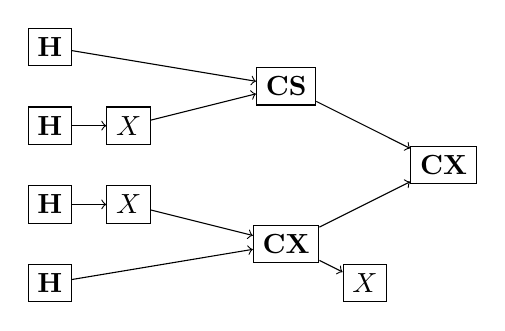
\begin{tikzpicture}
  \node[rectangle,draw] (A)  at (0,3) { $\mathbf{H}$ }; 
  \node[rectangle,draw] (B)  at (0,2) { $\mathbf{H}$ }; 
  \node[rectangle,draw] (C)  at (0,1) { $\mathbf{H}$ }; 
  \node[rectangle,draw] (D)  at (0,0) { $\mathbf{H}$ }; 
  \node[rectangle,draw] (E) at (1,2) { $\inr{X}$ } ; 
  \node[rectangle,draw] (F) at (1,1){ $\inr{X}$ }  ; 
  \node[rectangle,draw] (G)  at (3,2.5) { $\mathbf{CS}$ }; 
  \node[rectangle,draw] (H)  at (3,0.5) { $\mathbf{CX}$ }; 
  \node[rectangle,draw] (I)  at (4,0) { $\inr{X}$ }; 
  \node[rectangle,draw] (J)  at (5,1.5) { $\mathbf{CX}$ }; 
  \draw[->] (B) to (E);
  \draw[->] (C) to (F);
  \draw[->] (A) to (G);
  \draw[->] (E) to (G);
  \draw[->] (F) to (H);
  \draw[->] (D) to (H);
  \draw[->] (H) to (I);
  \draw[->] (G) to (J);
  \draw[->] (H) to (J);
\end{tikzpicture}
\end{minipage}
\caption{  Example of a subjected quantum circuit: the even layers (0, 2, 4) contain the original gates, while the faults are imposed on the odd layers and marked in red. }
  \label{fig:examplecirc}
\end{figure}


The advantage of the barrier formulation is that we need not assign a useful probability directly to a nontrivial logical cycle with no syndrome. We instead bound the probability of the \emph{first appearance of a large connected syndrome} somewhere in the partially executed circuit. Such a syndrome leaves a trace in a space--time contour, allowing us to reason about the faults that created it.

\paragraph{The encoded computation and the role of logical gates.}
We next explain which circuit histories the contour argument must handle. As in standard fault-tolerance constructions, encoded zeros and encoded resource states are prepared in an initialization stage, for which we invoke existing fault-tolerant methods \cite{aharonov1999faulttolerant,gottesman2014faulttolerant,grospellier:tel-03364419}. Thereafter each logical register is encoded in a 4D Toric code. At the level of the encoded computation we interleave constant-depth sweep cycles with logical operations from the universal set
\begin{equation*}
  \mathbf X,\ \mathbf Z,\ \mathbf{CX},\ \mathbf H,\ \mathbf S,\ \mathbf T.
\end{equation*}
Logical Paulis and controlled-NOT admit transversal implementations. The remaining gates are implemented by gate teleportation with encoded resource states \cite{Zhou_2000}. The role of teleportation is important for the proof: the circuit can carry out a logical operation without introducing an uncontrolled large spatial deformation of the error chain.

Informally, a gate-teleportation gadget couples the data register to an appropriate resource state, measures the relevant input registers, and computes a logical measurement result from the classical outcomes. Depending on that result, it performs a Pauli correction or another prescribed feed-forward operation. The classical decoding may take more than one physical time step. During this waiting period the quantum register that carries the output continues to undergo ordinary sweep cycles; the correction rule is not replaced by a more elaborate decoder. For the relevant $X$-basis measurement we use a fold-transversal Hadamard realization \cite{Breuckmann_2024}; its use at measurement need not preserve the geometric extent of a register that will subsequently be discarded. In the detailed proof, we track how Pauli chains and their boundary chains propagate through these gadgets (\Cref{subsection:logical}).

This leads to a useful distinction among the layers in a contour history: a sweep-correction layer, a layer of faults, and a layer implementing a logical operation need not obey the same geometric estimate. Only the sweep provides a guaranteed strict decrease in the designated potential; logical operations are designed not to produce uncontrolled growth, while faults can introduce new syndrome witnesses. The explanation-tree induction keeps track of these different cases instead of treating all layers as identical.

\paragraph{The quantum Toom contour: what its vertices mean.}
We now construct the analogue of the classical contour from the actual error history of the encoded circuit. Fix a realization of the Pauli faults and the measurement outcomes. Propagating the faults through the conditioned circuit gives a sequence of Pauli errors $P_1,P_2,\ldots$, one for each time boundary. Represent the $X$ part of each Pauli by a chain on the infinite cubical cover and the $Z$ part by a chain on the dual cover. The \emph{syndrome} of either chain is its boundary. We are interested in the vertices that \emph{witness} a nonzero syndrome: a lattice vertex witnesses the syndrome when it belongs to a face in the support of the boundary chain.

The space--time contour is a graph $\mathcal H=(V_{\mathcal H},E_{\mathcal H})$ constructed as follows. We describe the rules informally here; the formal graph also records the encoded register and whether a vertex belongs to the $X$ or $Z$ syndrome sector.
\begin{enumerate}
  \item \emph{Syndrome witnesses.} Include a vertex $(v,t)$ when the vertex $v$ witnesses a nonzero syndrome at time $t$. An erroneous qubit whose error is a stabilizer may therefore contribute no contour vertex at all.
  \item \emph{Arrows.} When an update can carry the influence of a witness $(u,t)$ to a witness $(v,t+1)$, connect them by a directed, time-respecting arrow. The endpoints lie within a bounded neighborhood in the space--time base graph; for a gate coupling different encoded registers, the arrow can connect the corresponding registers.
  \item \emph{Forks and leaves.} Record additional local connections between witnesses with a common successor, so that histories explaining the same future syndrome are not treated as unrelated. These are the forks. Vertices whose history does not continue backward through arrows are charged to the creation of syndrome by faults (or to the noisy initialization); they play the role of leaves in an explanation.
\end{enumerate}
The figure below shows a sweep of a small error cluster and the corresponding pattern of arrows and forks. The contour records \emph{which syndrome witnesses could have caused which later witnesses}; it is not simply the diagram of qubits that carry Pauli errors.


\begin{figure}[h]
  \centering
  \ifdefined \POSTER \begin{tikzpicture}[scale=4] \else \begin{tikzpicture}[scale=1.5] \fi

\tikzset{xyp/.style={canvas is xy plane at z=#1}}
\tikzset{xzp/.style={canvas is xz plane at y=#1}}
\tikzset{yzp/.style={canvas is yz plane at x=#1}}



\draw[green!20!black,fill=green!70!black!70,rounded corners=1,opacity=0.5, xzp=0]%,shift={(0.15,0.15)}]
(-0.1,2.1) rectangle (1.1,0.9);

\draw[green!20!black,fill=green!70!black!70,rounded corners=1,opacity=0.5, xzp=1]%,shift={(0.15,0.15)}]
(0.9,2.1) rectangle (2.1,0.9);

      \draw[green!20!black,fill=green!70!black!70,rounded corners=1,opacity=0.5, yzp = 0]%,shift={(0.15,0.15)}]
      (-0.1,2.1) rectangle (1.1, 0.9);


      \draw[green!20!black,fill=green!70!black!70,rounded corners=1,opacity=0.5, xyp = 2]%,shift={(0.15,0.15)}]
      (-0.1,-0.1) rectangle (1.1, 1.1);
      

      \draw[green!20!black,fill=green!70!black!70,rounded corners=1,opacity=0.5, yzp = 1]%,shift={(0.15,0.15)}]
      (-0.1,2.1) rectangle (1.1, 0.9);
%,opacity=0.5]
%\fill[green!30]
%(0.8,0.8,1.2) -- (0.7,0.7,0) -- (2,2,0) -- (2,2,1.2) -- cycle;
%
%\fill[green!30]
%(0.9,0.9,1.1) -- (0.9,0.9,-0.1) -- (1.1,0.9,-0.1) -- (1.1,0.9,1.1) -- cycle;  



      \draw[blue, thick]  (0,1,2) -- (1,1,2); % -- (1,1,1);
      \draw[blue, thick] (0,1,1) -- (0,1,2) -- (0,1,1) -- (0,0,1) -- (1,0,1) -- (1,1,1) -- (2,1,1) -- (2,1,2) -- (1,1,2);


      \node[below , scale=0.7] at (0,1,2) { $(v_{1}, t)$ } ;
      \node[below , scale=0.7] at (0,1,1) {$(v_{2}, t)$} ;
      \node[below , scale=0.7] at (0,0,1) {$(v_{3}, t)$} ;
      \node[below , scale=0.7] at (1,0,1) {$(v_{4}, t)$} ;
      \node[below , scale=0.7] at (1,1,1) {$(v_{5}, t)$} ;
      \node[below , scale=0.7] at (2,1,1) {$(v_{6}, t)$} ;
      \node[below , scale=0.7] at (2,1,2) {$(v_{7}, t)$} ;
      \node[below , scale=0.7] at (1,1,2) {$(v_{8}, t)$} ;
% draw grid lines
\foreach \x in {0,1,2} {
  \foreach \y in {0,1,2} {
    \draw[gray] (\x,\y,0) -- (\x,\y,2);
  }
}

\foreach \x in {0,1,2} {
  \foreach \z in {0,1,2} {
    \draw[gray] (\x,0,\z) -- (\x,2,\z);
  }
}

\foreach \y in {0,1,2} {
  \foreach \z in {0,1,2} {
    \draw[gray] (0,\y,\z) -- (2,\y,\z);
  }
}

% draw lattice points
\foreach \x in {0,1,2} {
  \foreach \y in {0,1,2} {
    \foreach \z in {0,1,2} {
      \fill (\x,\y,\z) circle (1pt);
    }
  }
}

\draw (2.5,1) node { $\rightarrow$ };
\end{tikzpicture} \ifdefined \POSTER \begin{tikzpicture}[scale=4] \else \begin{tikzpicture}[scale=1.5] \fi
\tikzset{xyp/.style={canvas is xy plane at z=#1}}
\tikzset{xzp/.style={canvas is xz plane at y=#1}}
\tikzset{yzp/.style={canvas is yz plane at x=#1}}



\draw[green!20!black,fill=green!70!black!70,rounded corners=1,opacity=0.5, xzp=0]%,shift={(0.15,0.15)}]
(-0.1,2.1) rectangle (1.1,0.9);

\draw[green!20!black,fill=green!70!black!70,rounded corners=1,opacity=0.5, xzp=1]%,shift={(0.15,0.15)}]
(0.9,2.1) rectangle (2.1,0.9);

      \draw[green!20!black,fill=green!70!black!70,rounded corners=1,opacity=0.5, yzp = 0]%,shift={(0.15,0.15)}]
      (-0.1,2.1) rectangle (1.1, 0.9);


      \draw[green!20!black,fill=green!70!black!70,rounded corners=1,opacity=0.5, xyp = 2]%,shift={(0.15,0.15)}]
      (-0.1,-0.1) rectangle (1.1, 1.1);
      

      \draw[green!20!black,fill=green!70!black!70,rounded corners=1,opacity=0.5, yzp = 1]%,shift={(0.15,0.15)}]
      (-0.1,2.1) rectangle (1.1, 0.9);

\draw[green!20!black,fill=green!70!black!70,rounded corners=1,opacity=0.5, xzp=1]%,shift={(0.15,0.15)}]
(-0.1,2.1) rectangle (1.1,0.9);

      \draw[green!20!black,fill=green!70!black!70,rounded corners=1,opacity=0.5, xyp = 1]%,shift={(0.15,0.15)}]
      (-0.1,-0.1) rectangle (1.1, 1.1);


      \draw[blue, thick]  (1,1,1) -- (2,1,1) -- (2,1,2) -- (1,1,2) -- (1,1,1);

      \node[below , scale=0.7] at (0,1,2) { $(v_{1}, t+1)$ } ;
      \node[below , scale=0.7] at (0,1,1) {$(v_{2}, t+1)$} ;
      \node[below , scale=0.7] at (0,0,1) {$(v_{3}, t+1)$} ;
      \node[below , scale=0.7] at (1,0,1) {$(v_{4}, t+1)$} ;
      \node[below , scale=0.7] at (1,1,1) {$(v_{5}, t+1)$} ;
      \node[below , scale=0.7] at (2,1,1) {$(v_{6}, t+1)$} ;
      \node[below , scale=0.7] at (2,1,2) {$(v_{7}, t+1)$} ;
      \node[below , scale=0.7] at (1,1,2) {$(v_{8}, t+1)$} ;

% draw grid lines
\foreach \x in {0,1,2} {
  \foreach \y in {0,1,2} {
    \draw[gray] (\x,\y,0) -- (\x,\y,2);
  }
}

\foreach \x in {0,1,2} {
  \foreach \z in {0,1,2} {
    \draw[gray] (\x,0,\z) -- (\x,2,\z);
  }
}

\foreach \y in {0,1,2} {
  \foreach \z in {0,1,2} {
    \draw[gray] (0,\y,\z) -- (2,\y,\z);
  }
}

% draw lattice points
\foreach \x in {0,1,2} {
  \foreach \y in {0,1,2} {
    \foreach \z in {0,1,2} {
      \fill (\x,\y,\z) circle (1pt);
    }
  }
}
\end{tikzpicture}


\ifdefined \POSTER \begin{tikzpicture}[scale=4] \else \begin{tikzpicture}[scale=1.5] \fi


\tikzset{xyp/.style={canvas is xy plane at z=#1}}
\tikzset{xzp/.style={canvas is xz plane at y=#1}}
\tikzset{yzp/.style={canvas is yz plane at x=#1}}





\node(A) at (0,1,2) {} ;
\node(B) at (0,1,1) {} ;
\node(C) at (0,0,1) {} ;
\node(D) at (1,0,1) {} ;
\node(E) at (1,1,1) {} ;
\node(F) at (2,1,1) {} ;
\node(G) at (2,1,2) {} ;
\node(H) at (1,1,2) {} ;


      \fill (0,1,2) circle(1pt)  ;
      \fill (0,1,1) circle(1pt) ;
      \fill (0,0,1) circle(1pt) ;
      \fill (1,0,1) circle(1pt) ;
      \fill (1,1,1) circle(1pt) ;
      \fill (2,1,1) circle(1pt) ;
      \fill (2,1,2) circle(1pt) ;
      \fill (1,1,2) circle(1pt) ;
% draw grid lines

% draw lattice points
\foreach \x in {0,1,2} {
  \foreach \y in {0,1,2} {
    \foreach \z in {0,1,2} {
      \node at (\x,\y,\z) { } ;
    }
  }
}


\node[below , scale=0.7](I) at (5,1,1) {$(v_{5}, t+1)$} ;
\node[below , scale=0.7](J) at (6,1,1) {$(v_{6}, t+1)$} ;
\node[below , scale=0.7](K) at (6,1,2) {$(v_{7}, t+1)$} ;
\node[below , scale=0.7](L) at (5,1,2) {$(v_{8}, t+1)$} ;
 
\draw[blue,very thin,-> ]  (A) to [out=50, in=130] (I); 
\draw[blue,very thin,-> ]  (A) to [out=50, in=130] (L);
\draw[blue,very thin,-> ]  (B) to [out=50, in=130] (I); 
\draw[blue,very thin,-> ]  (B) to [out=50, in=130] (L);
\draw[blue,very thin,-> ]  (C) to [out=50, in=130] (I); 
\draw[blue,very thin,-> ]  (D) to [out=50, in=130] (I); 
\draw[blue,very thin,-> ]  (D) to [out=50, in=130] (L);
\draw[blue,very thin,-> ]  (E) to [out=50, in=130] (J); 
\draw[blue,very thin,-> ]  (E) to [out=50, in=130] (L);
\draw[blue,very thin,-> ]  (E) to [out=50, in=130] (K); 


\draw[blue,very thin,-> ]  (H) to [out=50, in=130] (I); 
\draw[blue,very thin,-> ]  (H) to [out=50, in=130] (K);
\draw[blue,very thin,-> ]  (H) to [out=50, in=130] (J); 

\draw[blue,very thin,-> ]  (F) to [out=50, in=130] (I); 
\draw[blue,very thin,-> ]  (F) to [out=50, in=130] (L);
\draw[blue,very thin,-> ]  (F) to [out=50, in=130] (K); 

\draw[blue,very thin,-> ]  (G) to [out=50, in=130] (I); 
\draw[blue,very thin,-> ]  (G) to [out=50, in=130] (L);
\draw[blue,very thin,-> ]  (G) to [out=50, in=130] (J); 

\draw[green,very thin,<-> ]  (A) to (B); 
\draw[green,very thin,<-> ]  (A) to (C); 
\draw[green,very thin,<-> ]  (A) to (D); 
\draw[green,very thin,<-> ]  (A) to (E); 
\draw[green,very thin,<-> ]  (A) to  (H);
\draw[green,very thin,<-> ]  (A) to  (G);
\draw[green,very thin,<-> ]  (A) to  (F);

\draw[green,very thin,<-> ]  (B) to (C); 
\draw[green,very thin,<-> ]  (B) to (D); 
\draw[green,very thin,<-> ]  (B) to (E); 
\draw[green,very thin,<-> ]  (B) to  (H);
\draw[green,very thin,<-> ]  (B) to  (G);
\draw[green,very thin,<-> ]  (B) to  (F);


\draw[green,very thin,<-> ]  (C) to (D); 
\draw[green,very thin,<-> ]  (C) to (E); 
\draw[green,very thin,<-> ]  (C) to  (H);
\draw[green,very thin,<-> ]  (C) to  (G);
\draw[green,very thin,<-> ]  (C) to  (F);

\draw[green,very thin,<-> ]  (D) to (E); 
\draw[green,very thin,<-> ]  (D) to  (H);
\draw[green,very thin,<-> ]  (D) to  (G);
\draw[green,very thin,<-> ]  (D) to  (F);

\draw[green,very thin,<-> ]  (E) to  (H);
\draw[green,very thin,<-> ]  (E) to  (G);
\draw[green,very thin,<-> ]  (E) to  (F);


\draw[green,very thin,<-> ]  (F) to  (H);
\draw[green,very thin,<-> ]  (F) to  (G);

\draw[green,very thin,<-> ]  (H) to  (G);


      \fill (5,1,1) circle(1pt) ;
      \fill (6,1,1) circle(1pt) ;
      \fill (6,1,2) circle(1pt) ;
      \fill (5,1,2) circle(1pt) ;

\node[below , scale=0.7] at (0,1,2) { $(v_{1}, t)$ } ;
\node[below , scale=0.7] at (0,1,1) {$(v_{2}, t)$} ;
\node[below , scale=0.7] at (0,0,1) {$(v_{3}, t)$} ;
\node[below , scale=0.7] at (1,0,1) {$(v_{4}, t)$} ;
\node[below , scale=0.7] at (1,1,1) {$(v_{5}, t)$} ;
\node[below , scale=0.7] at (2,1,1) {$(v_{6}, t)$} ;
\node[below , scale=0.7] at (2,1,2) {$(v_{7}, t)$} ;
\node[below , scale=0.7] at (1,1,2) {$(v_{8}, t)$} ;




% draw grid lines

% draw lattice points
      \foreach \x in {4,5,6} {
  \foreach \y in {0,1,2} {
    \foreach \z in {0,1,2} {
      \node at  (\x,\y,\z) { };
    }
  }
}
\end{tikzpicture}


\caption{
Above: The application of a sweep-cycle, where the green faces represent the bits assignment $z$, and the blue edges correspond to unsatisfied checks $\partial^{-} z$. The vertices witnessing a syndrome, namely belonging to $\partial^{-}z$, are labeled as $v_{1}, v_{2}, \ldots, v_{8}$. Notice that the leftmost bottom-inner vertex is not witnessing a syndrome even though it belongs to $z$. Below: The Toom's contour derived from the single computation layer that matches the cycle. Arrows are colored in blue, while forks are colored in green. Note that $(v_{1}, t+1)$ doesn't belong to the Toom's contour (since $v_{1}$ doesn't see an unsatisfied check at time $t+1$).
}
  \label{fig:toomscontours}
\end{figure}


There is a subtle reason for taking vertices witnessing \emph{syndromes} rather than erroneous qubits as the nodes of our graph. A stabilizer can have large physical support and still be harmless, and the sweep rule need not remove it because it has no syndrome to act upon. Tracking all Pauli errors as classical ``wrong bits'' would charge the analysis for such harmless errors. Tracking the boundary chain instead respects the homological equivalence built into the code. This is where the geometric content of the chain complex enters the probabilistic argument, not merely the definition of the local correction.

\paragraph{Slices, poles, and predecessor decompositions.}
A contour can have many components, branching in both space and time. To bound a particular late-time syndrome, we work with \emph{slices}: roughly, the parts of the contour at a fixed time that are grouped together by the arrow structure. Each slice has a geometric size, defined using the potential walls of its witnesses after projection to the same infinite lattice. A slice of size $s$ has, for each of the $d+1$ potentials, a point attaining its maximum. We call a choice of these points a \emph{pole selection}. The same physical vertex may be a pole for several potentials.

Consider a slice $K$ at time $t+1$ and choose its poles. For every selected pole that was not itself created by a new fault, follow one of its possible arrows back to a witness at time $t$. The predecessors may lie in several different slices $K_0,\ldots,K_k$. We add just enough forks to connect the predecessor slices that are needed to account for the chosen poles. This gives a \emph{predecessor decomposition} of $K$. The reason for choosing poles, rather than trying to preserve every vertex of $K$, is that the poles determine the geometric size we need to estimate. Consequently, the predecessor decomposition can be kept small while still retaining the information relevant to the bound.

The decomposition has two important properties. First, predecessor slices reached through different arrow components have disjoint backward histories, so their marked fault leaves can be counted separately. Second, the size of $K$ is controlled by the sum of the sizes of its predecessor slices and the lengths of the connecting forks. Forks have bounded spatial size because all physical operations have bounded support and the code dimension is fixed. Moreover, for a slice immediately following a sweep cycle, the deterministic shrinking result strengthens the predecessor inequality by \emph{one unit}. Schematically, if $s$ is the selected-pole size of $K$ and $s_j$ are the corresponding sizes of its predecessors, the estimates have the form
\begin{equation*}
 \sum_{j=0}^{k}s_j+\sum_{j=1}^{k}\operatorname{Size}(F_j)
 \ \geq\
 \begin{cases}
   s+1,&\text{when $K$ follows a sweep cycle},\\
   s,&\text{for the other ordinary layer types}.
 \end{cases}
\end{equation*}
This is the link between the geometric shrinking lemma and a combinatorial count of faults. The formal predecessor and layer-dependent estimates appear in \Cref{subsection:spacetimegraph}.

\paragraph{What is an explanation tree, and why does it have many leaves?}
We can finally make the backwards-history idea precise enough to see how the probability estimate works. Start from the poles of a slice $K$ and apply its predecessor decomposition. For each predecessor slice, repeat the same operation. Every time we go backward through an arrow we learn where the relevant syndrome could have come from; every fork allows us to join two pieces of that history. The recursion ends at witnesses attributable to faults. The resulting connected subgraph is an \emph{explanation} of the original slice. By deleting redundant edges, we may take a spanning tree of this explanation. Its terminal marked vertices are its \emph{fault leaves}; the other vertices and edges provide the causal paths from those faults to the poles of $K$.

An explanation tree does not mean that the faults themselves form a tree in physical space. Rather, the \emph{dependencies among syndrome witnesses at different times} contain a tree. Two errors introduced far apart can have histories that meet after several rounds; the forks explicitly record such mergers. Conversely, a large cluster observed at a late time cannot be credited to one arbitrarily influential fault, because a bounded-support operation reaches only a bounded neighborhood per time step and a sweep erodes geometric extent. These observations are formalized through an induction on the height of the history.

The induction maintains two kinds of information at once: the number $m$ of marked fault leaves and the numbers of arrows and forks required to connect them to the selected poles. At a newly created witness the explanation consists of one leaf. At a later slice, take explanations of the predecessor slices, add arrows from the new poles to their predecessors, and join these components using the selected forks. Disjoint predecessor histories let us add their leaf counts. The geometric predecessor inequality, including the one-unit improvement at sweep layers, pays for the extra edges introduced at each step. A layer-dependent version of this invariant gives constants $\alpha,\beta>0$ (depending only on $d,d'$) such that, schematically,
\begin{equation*}
  |A|\ \leq\ \alpha(m-c_r)-\beta s,
  \qquad |F|\ \leq\ m-1,
\end{equation*}
where $A$ and $F$ are the arrows and forks of the explanation, and $c_r$ is a fixed constant depending on the type of the last layer. In particular, the estimate forces the explanation to contain a number of leaves proportional to $s$ and prevents its number of edges from being arbitrarily large compared with the number of leaves. This is the \emph{minimal-explanation argument} of \Cref{subsection:explantion}. We emphasize that the word ``minimal'' refers to a controlled connected explanation of the relevant poles, not to an optimization algorithm that searches all possible histories.

\paragraph{The infinite cover and distinct physical faults.}
A last issue arises when we turn the leaves into a probability. We built the geometry in $\mathbb Z^d$, but actual noise acts on the \emph{finite} Toric complex. Points differing by a vector in $n\mathbb Z^d$ represent the same physical location. Therefore, several leaves of an explanation in the infinite cover might project onto the same physical faulty qubit. We cannot simply raise the noise rate $p$ to the total number of such leaves: the local-stochastic condition charges each \emph{distinct} physical fault location only once.

We address this by a combinatorial selection argument introduced in \cite{Berman}. The bounded-degree explanation contains a large subtree whose spatial spread is small compared with the torus side length, while retaining a constant fraction of the relevant leaf-to-edge ratio. Inside this subtree, distinct translated leaves can be matched to distinct physical fault locations (up to the fixed multiplicity associated with one faulty qubit). Thus, an explanation of a large slice certifies the occurrence of a \emph{linear number of distinct faults}, even though the original explanation was constructed in the periodic cover. This is the role of the tree-separator argument in the appendix. It is essential when passing from deterministic statements on the infinite lattice to probability bounds for the finite quantum circuit.

\paragraph{Why we must also analyze a partially executed final layer.}
Recall that the barrier is crossed at an \emph{elementary step}, not necessarily at the end of a complete correction or fault layer. A contour made only from complete time layers could miss the very configuration whose probability we wish to bound. We therefore define an analysis contour that agrees with the ordinary contour at all preceding completed times, but whose last layer records the propagated error after the selected intermediate step.

In this last layer we add local connections between syndrome witnesses meeting a common check. They ensure that a connected syndrome component at the barrier crossing appears as a connected object in the contour, even if the usual backward-arrow relation alone would split it into several pieces. These extra links are \emph{only} a device for the last partial layer: adding them throughout the history would change the predecessor structure on which the induction relies. Because each new connection has bounded spatial extent, the final-layer estimate is weaker by only a dimension-dependent constant, and the explanation-tree count still applies. The formal analysis contour is defined in \Cref{subsection:toricencoded}; its last-layer estimate is proved in \Cref{subsection:spacetimegraph,subsection:explantion}.

\paragraph{From explanation trees to a threshold.}
We now assemble the argument. Suppose a syndrome slice has geometric size $s$. The previous steps imply that its history contains an explanation with at least a constant multiple of $s$ \emph{distinct physical fault locations}, and that an explanation of $q$ edges requires at least a constant multiple of $s+q$ such locations. Since the underlying space--time graph has bounded degree, the number of possible connected explanations with $q$ edges rooted at a specified witness grows at most exponentially in $q$. On the other hand, the local-stochastic noise condition bounds the probability that every location in any predetermined set of $r$ distinct locations is faulty by $p^r$. Therefore the sum over candidate explanations is bounded by a convergent geometric series once $p$ is sufficiently small. In particular, the probability of a slice of geometric size at least $s$ decreases exponentially with $s$, up to the polynomial number of possible roots and observation times.

The barrier argument now turns this statement into fault tolerance. If an encoded computation suffers a logical error, some intermediate step must be the first to exhibit a connected syndrome component of size $\Omega(n)$. The analysis contour for that step contains a comparably large slice. The explanation estimate makes this event at most
\begin{equation*}
  O\!\left(\operatorname{poly}(w,\mu,n)\right)p^{\Omega(n)}
\end{equation*}
under sufficiently weak local-stochastic noise, where $w$ and $\mu$ are the width and depth of the ideal computation. Taking a union bound over the registers and steps establishes the desired bound for the encoded simulation (\Cref{theorem:main}). No independence between different fault locations, and no expansion inequality for the Toric complex, is used in this probability step.

\paragraph{Why the same method proves ideal decoding.}
There is one final application. Suppose an encoded state is subjected to a single, initially sampled local-stochastic Pauli error, and all subsequent sweep cycles are \emph{noiseless}. This is a different claim from maintaining a state during a long noisy computation: the aim now is to remove the initial error by repeated use of the sweep rule. If every relevant syndrome component stays below the geometric barrier, the deterministic shrinking argument guarantees that the syndrome eventually disappears. The barrier result also prevents the evolution from moving to a different logical class. A further counting argument bounds the probability that a barrier-sized slice ever appears during this noiseless evolution, treating the initially sampled fault set as the source of the contour leaves. After $n^{d+1}$ ideal sweep cycles the state is therefore recovered with probability at least
\begin{equation*}
  1-O\!\left(\operatorname{poly}(n)\right)p^{\Omega(n)},
\end{equation*}
as stated in \Cref{theorem:idealdec}.

Thus the two threshold statements share a single mechanism. \emph{Cubical chains} make the local sweep correction explicit and give a geometric shrinking property for syndrome boundaries. \emph{First barrier crossings} reduce logical failure to the appearance of a large intermediate syndrome. Finally, \emph{Toom-type explanations} show that such a syndrome would require too many prescribed faulty locations to be likely. The proof uses the geometry and homology of the Toric code in place of expansion, and it uses error histories rather than a per-round invariant asserting that the physical error itself remains sparse.

